\documentclass{article}
\usepackage[utf8]{inputenc}

\title{Report.7.reduce.tex}
\author{gw.muraro}
\date{November 1st 2018}

\usepackage{natbib}
\usepackage{graphicx}
\usepackage{pgfplots}
\usepackage{minted}

\begin{document}

\maketitle
\section{Labwork 7}

\subsection{Explain how you implement the labworks}

    The main goal of this labwork is to use reduction in order to get a minimal and a maximal value of the image and avoid simultaneous bank memory access. We will accomplish this by using different kernel functions and passing arrays that we will cache and reduce to have only one value of minimum and maximum. Then, we will use a map kernel function to adjust all the pixels of the image. 

    \begin{enumerate}     

    \item \textbf{First reduce}
    
    The goal of this kernel is to get a minimum and a maximum value of pixel intensity and put it into an array that will contains all min and max values per blocks. The corresponding kernel function is "reduceImage". 
    
    First, we have to use shared memory to get the gray value of our image. 
    \begin{minted}{c}
    
// getting the cache ID
int localtid = threadIdx.x; 
// getting the global ID
int tid = threadIdx.x + blockIdx.x * blockDim.x;

if (tid > imageWidth * imageHeight) return ;

// Make a cache array that contains the <BlockSize> value of gray
__shared__ int cacheMin[1024] ;
__shared__ int cacheMax[1024] ;	

// caching the gray values
cacheMin[localtid] = (in[tid].x + in[tid].y + in[tid].z)/3;
cacheMax[localtid] = (in[tid].x + in[tid].y + in[tid].z)/3;

__syncthreads();
    \end{minted}
    
    Now that we have our local Min and Max arrays, we can work on it. We will verify 2 by 2 the values of the array and keep the lower in the "localtid" index (the 0 value will compare to the $1024/2 = 512$). Then we will reduce by 2 the size of the array and do the same comparison until having only one minimal or maximal value. 
    
    \begin{minted}{c}
// reduction in cache
for (int s = blockDim.x / 2; s > 0; s /= 2) {
	// only processing the half lower values of the array
	if (localtid < s) {
		// compare 2 by 2
		cacheMin[localtid] = min(cacheMin[localtid], cacheMin[localtid + s]);
		cacheMax[localtid] = max(cacheMax[localtid], cacheMax[localtid + s]);
	}
	__syncthreads();
}
    \end{minted}
    
    Now, the cacheMin[0] value is the minimal value of the 1024 block. so we can put it into our global array (same for the max value) : 
    
    \begin{minted}{c}
// putting on global only for the first thread of the block 
if (localtid == 0){ 
    outMin[blockIdx.x] = cacheMin[0];
    outMax[blockIdx.x] = cacheMax[0];
}
    \end{minted}

    \item \textbf{Block reduction}
    
    We have now two arrays of the minimal and maximal values per blocks. We search now to have the minimal and maximal of all blocks. To do so, we use a loop in CPU. This loop's goal is pretty much the same as the previous loop in the kernel function : reduce the block number to 1. 
    
    \begin{minted}{c}
    
while(gridSize > 1) {
    // passing the output array as reduced input array to kernel functions
    reduceMin<<<gridSize, blockSize2>>>(devMin, devMin, inputImage->width, inputImage->height) ;
    reduceMax<<<gridSize, blockSize2>>>(devMax, devMax, inputImage->width, inputImage->height) ;
    gridSize = max(gridSize/blockSize2, 1);
}
    \end{minted}
    
    This block reduction is completed by a cache reduction in the kernel. The complete kernel function is the one below (reduceMin, reduceMax is similar) : 
    
    \begin{minted}{c}
__global__ void reduceMin(int * in, int * out, int imageWidth, int imageHeight) {	
    unsigned int localtid = threadIdx.x; // local id 
    unsigned int tid = threadIdx.x + blockIdx.x * blockDim.x;// global id 
    if (tid > imageWidth) return ;
	
    __shared__ int cache[1024] ;
    cache[localtid] = in[tid];
    __syncthreads();
	
    // reduction in cache
    for (int s = blockDim.x / 2; s > 0; s /= 2) {
        if (localtid < s) {
            cache[localtid] = min(cache[localtid], cache[localtid + s]);
        }
        __syncthreads();
    }		
	
    if (localtid == 0){ 
        out[blockIdx.x] = cache[0]; 
    }
}
    \end{minted}
    
    \item \textbf{Applying the stretch}
    From now, we have reduced all the values of the whole image pixels to 1 min and 1 max. We can now apply the map algorithm that is described below (and just being careful about the float division) : 
    
    \begin{minted}{c}
__global__ void stretch (
    uchar3 * devInput, 
    uchar3 * devOutput, 
    int imageWidth, 
    int imageHeight, 
    int minValue, 
    int maxValue) {
    
    //getting the pixel with the second dimension
    int tidx = (threadIdx.x + blockIdx.x * blockDim.x) ; 
    int tidy = (threadIdx.y + blockIdx.y * blockDim.y) ;

    if (tidx >= imageWidth || tidy >= imageHeight) return ;
    int tid = tidx + imageWidth * tidy ;
	
    /*IMPLEMENTATION*/
    devOutput[tid].x = (double(devInput[tid].x - minValue) 
                        / double(maxValue-minValue))*255;
    devOutput[tid].y = (double(devInput[tid].y - minValue) 
                        / double(maxValue-minValue))*255;
    devOutput[tid].z = (double(devInput[tid].z - minValue) 
                        / double(maxValue-minValue))*255;
}
    \end{minted}
    
    \end{enumerate}

\subsection{Results}
Since we use a 2D block size only for the map kernel function, the processing time is still high and could be optimize. These are the results :

    \begin{verbatim}
==== 2D Block Number : 2
USTH ICT Master 2018, Advanced Programming for HPC.
Warming up...
Starting labwork 7
labwork 7 ellapsed 32.9ms

==== 2D Block Number : 4
USTH ICT Master 2018, Advanced Programming for HPC.
Warming up...
Starting labwork 7
labwork 7 ellapsed 32.9ms

==== 2D Block Number : 16
USTH ICT Master 2018, Advanced Programming for HPC.
Warming up...
Starting labwork 7
labwork 7 ellapsed 28.6ms

==== 2D Block Number : 32
USTH ICT Master 2018, Advanced Programming for HPC.
Warming up...
Starting labwork 7
labwork 7 ellapsed 28.2ms
    \end{verbatim}

\subsection{Plot a graph}
    
   %%plot
    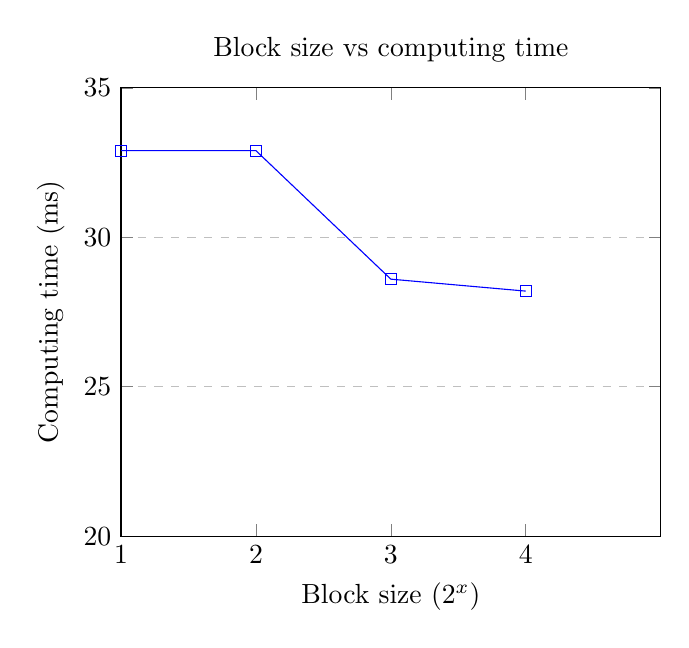
\begin{tikzpicture}
        \centering
        %%define axes
        \begin{axis}[
            title={Block size vs computing time},
            xlabel={Block size ($2^x$)},
            ylabel={Computing time (ms)},
            xmin=1, xmax=5,
            ymin=20, ymax=35,
            xtick={1, 2, 3, 4},
            ytick={20, 25, 30, 35},
            legend pos=north east,
            ymajorgrids=true,
            grid style=dashed,
        ]
        %% data filing
        \addplot[color=blue, mark=square]
            coordinates { %% Remind : axis X = 2^x
                (1,32.9)(2,32.9)(3,28.6)(4,28.2)
            };
        \end{axis}
    \end{tikzpicture}
    \newline


\end{document}

